%*******************************************************************************
%*********************************** Fifth Chapter *****************************
%*******************************************************************************

\chapter{Results and Discussions}  %Title of the Fifth Chapter

\section{Results}
    These are the different results of the experiments on the model. The indications of these results will then be discussed and analyzed.

    The first set of experiments will focus on the different cell dimensions as the experimental variable. The period and seasonality of data will be the controlled variables. The timestep will be set to monthly and the seasonality to false.

    \begin{table}[H]
      \centering
      \begin{tabular}{|c|c|c|c|}
            \hline
          \textbf{Cell Dimension}  &\textbf{MSE}  &\textbf{Accuracy} &\textbf{F1 Score}\\ 
          \hline
          500x500m &1.13 &88.98 &89.15 \\
          750mx750m &0.87 &91.78 &92.3 \\
          1000mx1000m  &0.98 &89.01 &90.36 \\
          \hline
        \end{tabular}
      \caption{Performance of the model for different cell dimensions}
    \end{table}
    Table 4.1 shows the results of the experiments for the different cell dimensions. The different cell dimensions are 500mx500m, 750mx750m, 1000mx1000m. The model performs highest with 750mx750m cell dimension with an accuracy of 91.78 and F1 score of 92.3.

    The next set experiments will focus on the different timesteps. The cell dimension and seasonality will now be controlled variables. The cell dimension will be set to 1000mx1000m and the seasonality to false.

    \begin{table}[H]
      \centering
      \begin{tabular}{|c|c|c|c|}
            \hline
          \textbf{Period}  &\textbf{MSE}  &\textbf{Accuracy} &\textbf{F1 Score}\\ 
          \hline
          Weekly &1.21 &87.74 &88.23 \\
          Monthly &0.67 &90.11 &89.54 \\
          Yearly   &0.98 &88.17 &89.10 \\
          \hline
        \end{tabular}
      \caption{Performance of the model for different timesteps}
    \end{table}
    Table 4.2 shows the results of the experiments for the different timesteps. The difference timesteps are weekly, monthly and yearly. The model performs highest with monthly timestep with an accuracy of 90.11 and F1 score of 89.54.

    The next set of experiments will focus on the seasonality of crime. The cell dimension and period will now be controlled variables. The cell dimension will be set to 1000mx1000m and the timestep to monthly.

    \begin{table}[H]
      \centering
      \begin{tabular}{|c|c|c|c|}
            \hline
          \textbf{Seaonality}  &\textbf{MSE}  &\textbf{Accuracy} &\textbf{F1 Score}\\ 
          \hline
          True &1.01 &89.15 &91.06\\
          False  &1.29 &89.62 &87.93 \\
          \hline
        \end{tabular}
      \caption{Performance of the model for seasonal and non-seasonal data}
    \end{table}
    Table 4.3 shows the results of the experiments for the seasonal (True) and non-seasonal data (False). Using seasonal data, the model performs at 89.15 accuracy and 91.06 F1 score. Using non-seasonal data, the model has almost the same accuracy of 89.62. The F1 score though is lower at 87.93.

\section{Discussions}

    \begin{figure}[H]
    \centering
    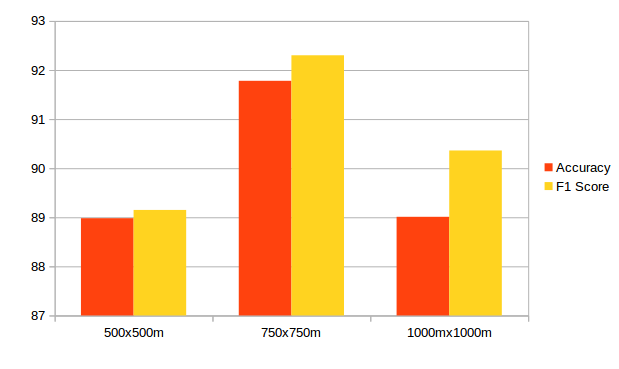
\includegraphics[width=12cm]{dimensions-experiments}
    \caption{Comparison of the Accuracy and F1 Score of the model for different cell dimensions.}
    \end{figure}
    The graph shown in Figure 4.1 compares the accuracy and F1 score of the model for the different cell dimensions. As can be seen, the model in 750mx750m cell dimension performs better in both metrics. The model in 500mx500m cell dimension has almost the same accuracy with the model in 1000mx1000m, with the latter having a higher F1 score.

    \begin{figure}[H]
    \centering
    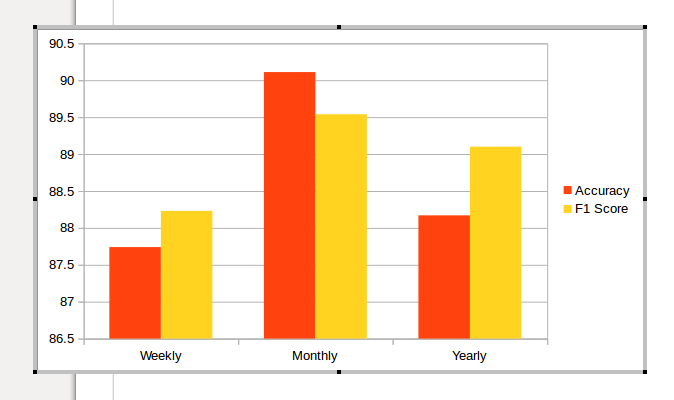
\includegraphics[width=12cm]{timestep-experiment}
    \caption{Comparison of the Accuracy and F1 Score of the model for timesteps.}
    \end{figure}
    Figure 4.2 above compares the accuracy and F1 score of the model for the different timesteps. The model in monthly timestep performs better in both accuracy and F1 score while the model in weekly timestep performs the worst.
    
    \begin{figure}[H]
    \centering
    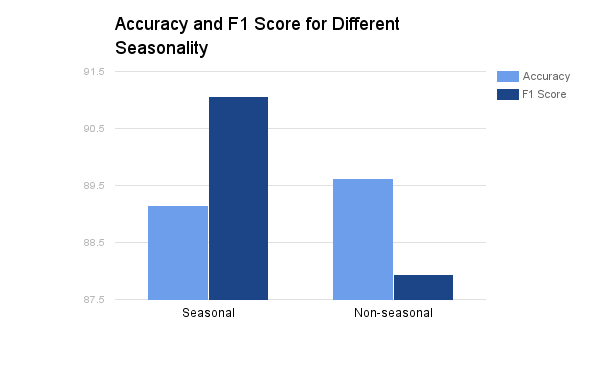
\includegraphics[width=12cm]{seasonal-experiments}
    \caption{Comparison of the Accuracy and F1 Score of the model for seasonal and non-seasonal data.}
    \end{figure}
    Figure 4.3 above compares the accuracy and F1 score of the model for seasonal and non-seasonal data. The model using seasonal data performs a little better in terms of F1 score compared to the model using non-seasonal data. The accuracy of both models have little difference.

\section{Error Analysis}
    To evaluate the performance of the model, error analysis was performed by plotting learning curves of the model's training error and cross-validation error for different timesteps. Through these curves, it can be determined whether the model suffered from variance error or bias error.

    \begin{figure}[H]
    \centering
    \begin{subfigure}{.5\textwidth}
      \centering
      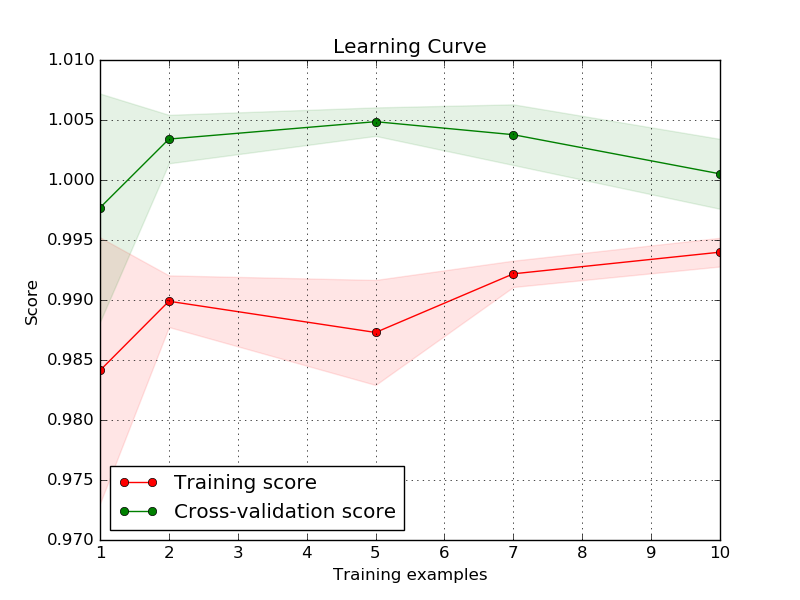
\includegraphics[width=1\linewidth]{500-yearly}
      \caption{500mx500m, yearly}
    \end{subfigure}%
    \begin{subfigure}{.5\textwidth}
      \centering
      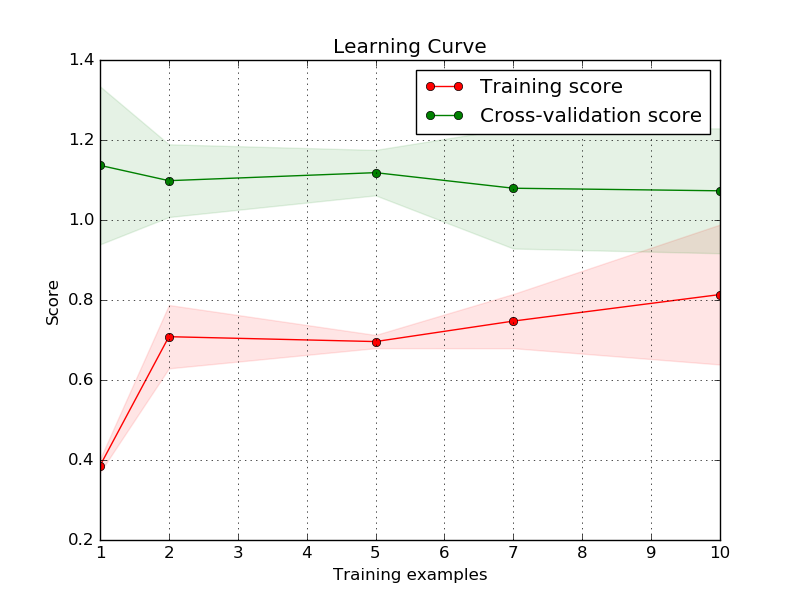
\includegraphics[width=1\linewidth]{1000-yearly}
      \caption{1000mx1000m, yearly}
    \end{subfigure}
    \caption{Learning curves of the model in different cell dimensions for the same timestep}
    \end{figure}

    Figure 4.4 shows the different learning curves of the model in different cell dimensions for the same timestep. The behavior of the training error and cross-validation error in both learning curves are almost similar, they tend to converge at the end but they have big gaps between them. Both instances of the model suffer from high variance. This may be because the yearly timestep yields only up to 16 samples with only 10 available for training. This low training sample size makes the model overfit. To reduce overfitting, more training examples must be used when using a yearly timestep, or use a different value for the timestep that yields bigger sample size. This explains why the monthly timestep performs better than the yearly timestep as shown in the results before. The graph shows that the variance or bias of the model is not affected by the cell dimension used.

    \begin{figure}[H]
      \centering
      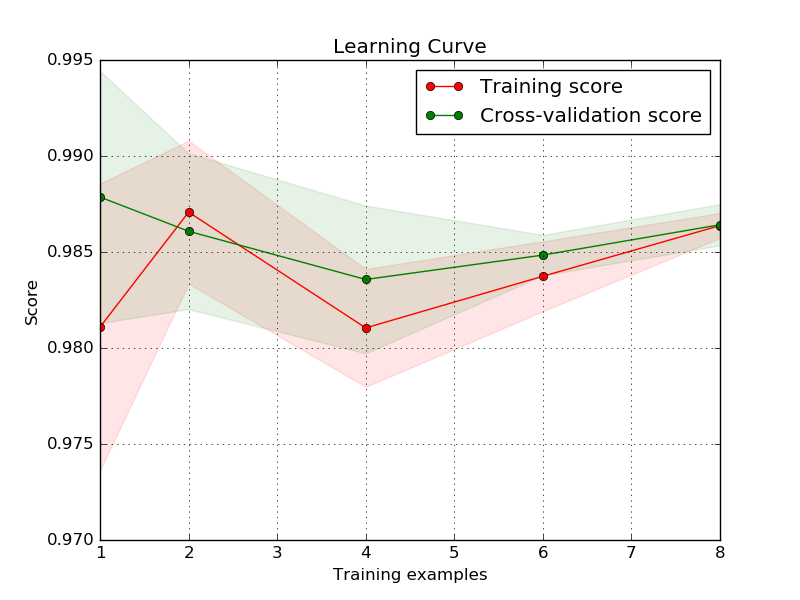
\includegraphics[width=10cm]{1000_weekly_False}
      \caption{Learning curve of the model in 1000mx1000m cell dimension and weekly timestep}
    \end{figure}
    Figure 4.5 shows the graph of the training error and cross-validation error of the model in a 1000mx1000m cell dimension and weekly timestep. Compared to the same model but with yearly timestep, this model suffers from high bias. The training error and cross-validation overlap each other and are almost of the same value. Weekly timestep, on the contrary to yearly timestep, yields a lot of data with respect to the number of features used. The model under this condition will underfit and fail to generalize the data. To reduce underfitting, more features must be fed to the model so that it can have more input to help it generalize data better.
